\chapter{Software Quality}
\label{squality}

\section{Application Summary}

The following is a summary of the various metrics of the application. A detailed breakdown by package in contained within the appendices.

\begin{table}[H]
\begin{center}
    \begin{tabular}{| l | l | l | l | p{2.3cm} |}
    \hline
    Metric & Total & Mean & Std. Deviation & Maximum\\ \hline
	McCabe Cyclomatic Complexity & n/a & 1.262 & .862 & 8\\ \hline
    
    \end{tabular}
\end{center}
\caption{Application Metrics}
\end{table}


\section{Software Quality Tools and Visualisations}

\begin{figure}[H]
\begin{center}
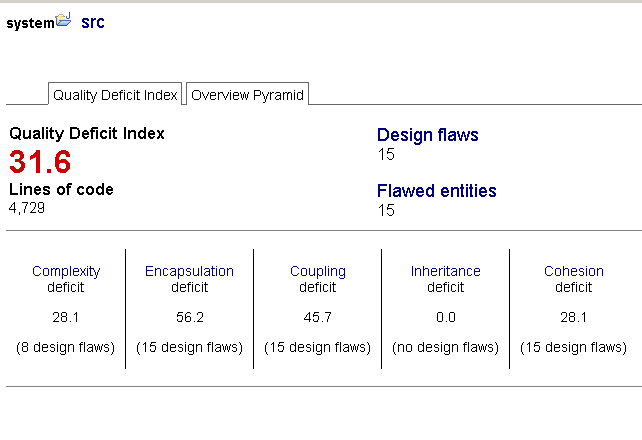
\includegraphics[scale=0.7]{infusion1.PNG}
\end{center}
\caption{Pre Re-factoring using Infusion}
\end{figure}

\begin{figure} [H]
\begin{center}
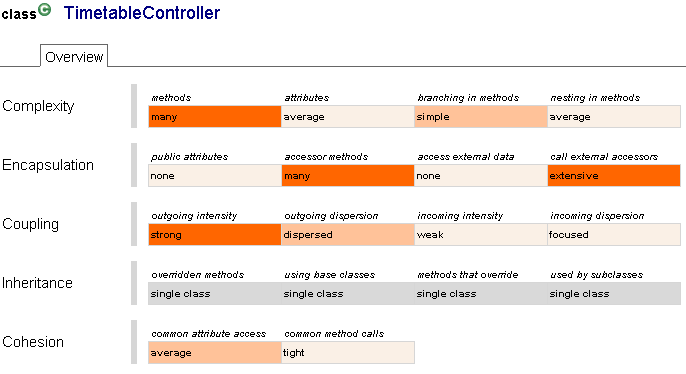
\includegraphics[scale=0.7]{infusion3.PNG}
\caption{Example of Class 'Bad Code Smell' Breakdown using Infusion}
\end{center}
\end{figure}

\begin{figure}[H]
\begin{center}
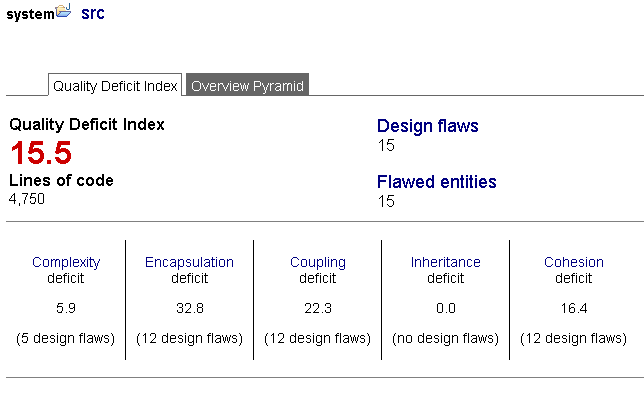
\includegraphics[scale=0.7]{infusion2.PNG}
\caption{Post Re-factoring using Infusion}
\end{center}
\end{figure}

\begin{figure}[H]
\begin{center}
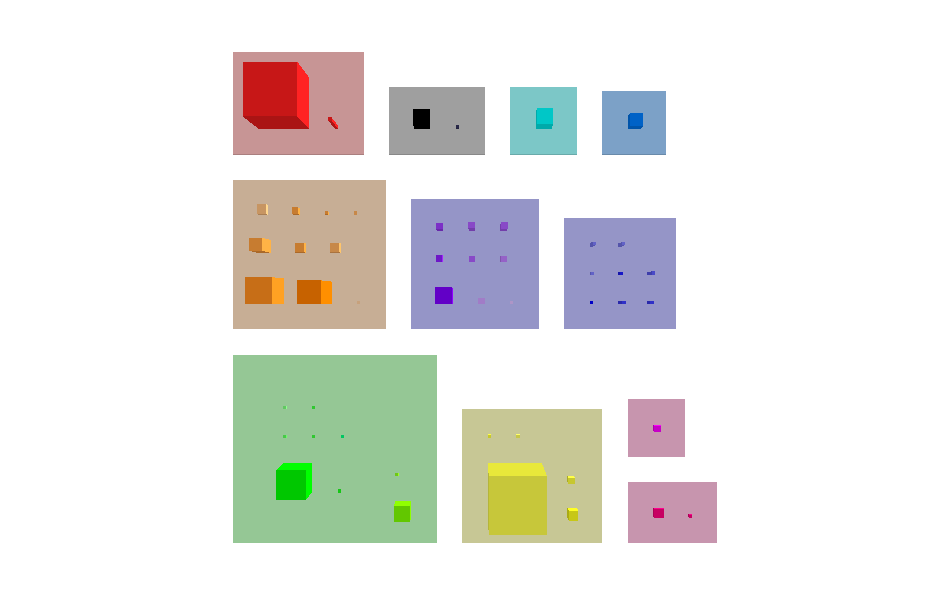
\includegraphics[scale=0.5]{codecity2d.png}
\caption{CodeCity 2D Visualisation of Application}
\end{center}
\end{figure}

\begin{figure}[H]
\begin{center}
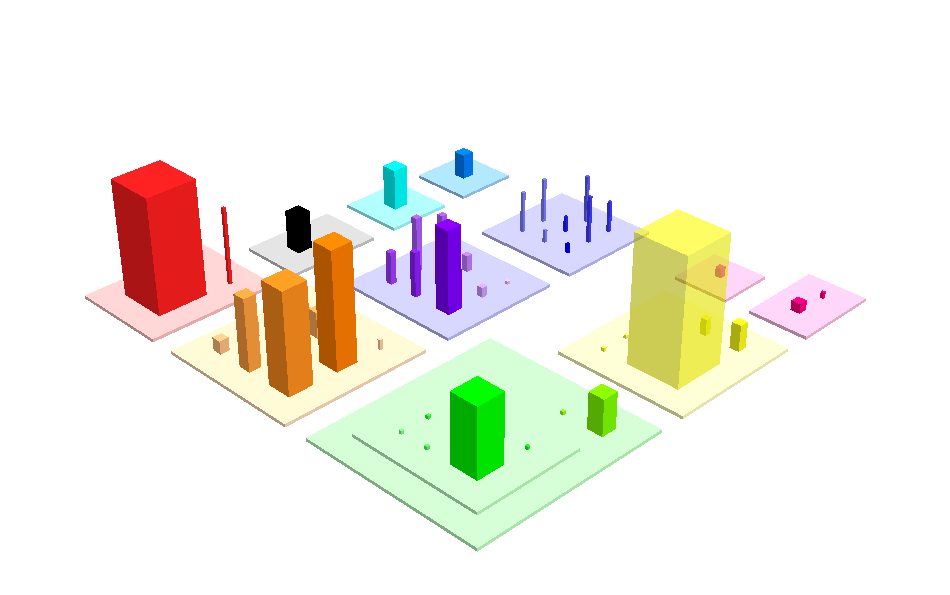
\includegraphics[scale=0.5]{codecity3d.png}
\caption{CodeCity 3D Visualisation of Application}
\end{center}
\end{figure}



\section{Sample Refactorings}
